\documentclass{myarticle}

\title{\textbf{\href{http://dx.doi.org/10.1680/geot.1963.13.2.147}{Effect of Aging of the Shear-Strength Properties of a Normally Consolidated Clay}\\时效对正常固结黏土抗剪强度特性的影响}}
\date{\today}
\author{Laurits Bjerrum \and K. Y. Lo}

\begin{document}

\maketitle

\section*{Synopsis 概要}

\begin{paracol}{2}

    In the Paper is described a series of triaxial tests on samples which were normally consolidated for different periods of time prior to the subsequent shear test. It is shown that the behaviour of the clay when sheared depends on the "age" of the samples. With time the clay becomes more brittle with smaller failure strains and the undrained shear strength shows a slight increase. A study of the stress-strain curves leads to the conclusion that the effect of time can be explained by the growing of cohesive bonds at the contact points between the particles. The cohesive bonds lead to a greater resistance against a shear deformation, but they are gradually destroyed for increasing strain.

    \switchcolumn

    在本文中,描述了对样品的一系列三轴试验,这些试验通常在随后的剪切试验之前的不同时间段内进行固结。结果表明,黏土在剪切时的行为取决于样品的“年龄”。 随着时间的流逝,黏土变得更脆,破坏应变较小,不排水的剪切强度略有增加。 对应力-应变曲线的研究得出的结论是,时间的影响可以通过颗粒之间接触点的粘聚力的增长来解释。 粘聚力导致对剪切变形的更大抵抗力,但是它们逐渐被破坏从而增加应变。

\end{paracol}

\section{Introduction 介绍}

\begin{paracol}{2}

    As a part of a current research on the stress-strain properties of normally consolidated clays an investigation has been made on the influence of the time on the undrained shearstrength and pore-pressure characteristics of a normally consolidated clay.

    \switchcolumn

    作为对正常固结黏土的应力-应变特性的当前研究的一部分,已经研究了时间对正常固结黏土的不排水剪切强度和孔隙压力特性的影响。

    \switchcolumn*

    There are two different ways in which the time factor may influence the results obtained by a conventional triaxial shear test. In the first place it is a well-known fact that the rate of application of the shear stresses has an influence on the shear strength of certain clay and shale \citep{Casacrande1951}.

    \switchcolumn
        
    时间因素可以通过两种不同的方式影响通过常规三轴剪切试验获得的结果。 首先,众所周知的事实是,剪切应力的施加速率会影响某些黏土和页岩的剪切强度\citep{Casacrande1951}。

    \switchcolumn*
    
    Recent research \citep{Bjerrum1958148} has, however, shown that in the second place a clay will behave differently depending on how long a time it has been left in the triaxial cell for consolidation. This means that samples consolidated for different periods of time prior to the shear testing might behave differently during a subsequent shear test depending on the "age" of the sample.

    \switchcolumn
            
    然而,最近的研究\citep{Bjerrum1958148}表明,在第二个位置,黏土的行为会有所不同,这取决于将其留在三轴单元中进行固化的时间。 这意味着在剪切试验之前经过不同时间合并的样品在随后的剪切试验中可能会根据样品的“年龄”而表现不同。

    \switchcolumn*

    In the above-mentioned Paper it was, for instance, shown that clays which exhibit secondary consolidation will gain in shear strength with time. But also clays which do not show a secondary time effect might change their properties with time and the tests described in the Paper indicated that with time a clay might become more brittle, showing lower strains at failure.

    \switchcolumn
        
    例如,在上述论文中,显示出二次固结的黏土的抗剪强度会随时间增加。 但是,未表现出二次时间效应的黏土也可能随时间改变其性能,并且本文所述的试验表明,随着时间的推移,黏土可能会变得更脆,显示出较低的破坏应变。

    \switchcolumn*

    This last-mentioned effect of time is of special interest for an evaluation of the undrained shear strength of normally consolidated clays. As pointed out in various Papers \citep{Bjerrum1960711, Bjerrum196123a}, there is a serious disagreement between the undrained shear strengths measured on undisturbed clay and on samples which have been reconsolidated in the laboratory. A possible explanation of this discrepancy may eventually be that an undisturbed clay since its deposition has gained some properties which cannot be reproduced in the laboratory where the time for which the sample is consolidated is of the order of a few days only. A reference should here be given to a previous study of this problem, made by \citet{Taylor195363}.

    \switchcolumn
        
    最后提到的时间影响对于评估正常固结的黏土的不排水剪切强度特别有意义。 正如各种论文所指出的那样\citep{Bjerrum1960711, Bjerrum196123a},在未经扰动的黏土上测量的不排水剪切强度与在实验室中重新固结的样品之间存在着严重的分歧。 这种差异的最终解释可能是未受干扰的黏土,因为其沉积获得了某些特性,而在实验室中,样品固结的时间只有几天左右,这些特性无法在实验室中再现。 这里应该参考以前由\citet{Taylor195363}进行的研究。

    \switchcolumn*

    With the purpose of investigating this factor a series of triaxial tests were performed in which samples of a normally consolidated clay, which did not show an appreciable secondary time effect, were sheared after different periods of aging. It is the results of this senes of tests which will be described below.

    \switchcolumn

    为了研究该因素,进行了一系列三轴试验,其中在不同的老化时间后剪切了未显示明显的二次时间效应的正常固结黏土样品。 这些感觉的结果将在下面描述。
    
\end{paracol}
\section{Properties Of The Clay 黏土的物理特性}

\begin{paracol}{2}

    The clay used for this study is a normally consolidated marine clay located at a place called Skabo, 2 miles west from the centre of Oslo. The undisturbed samples were obtained by the Norwegian Geotechnical Institute's thin-walled stationary piston sampler recovering samples of 80 cm long and 54 mm dia. In order to ensure homogeneity of the material used for the testing, the samples were taken from the same depths, 15-16 m, in eight boreholes made in the same vicinity.

    \switchcolumn

    这项研究使用的黏土是一种普通固结的海洋黏土,位于奥斯陆市中心以西2英里处的Skabo。 不受干扰的样品是由挪威地质技术研究所的薄壁固定式活塞取样器获得的,回收的样品长80厘米,直径54毫米。 为了确保试验所用材料的均匀性,从15-16m的相同深度的样品中,在附近进行了八个钻孔。

\end{paracol}

\begin{table*}[!htb]
    \centering
    \caption{Properties of Skabo clay}
    \addtocounter{table}{-1}
    \vspace{-8pt}
    \renewcommand{\tablename}{表}
    \caption{Skabo黏土的物理特性}
    \vspace{4pt}
    \renewcommand{\tablename}{Table}
    \begin{tabular}{ll|ll}
        \Xhline{1pt}
        Properties & value & Properties & value \\
        \Xcline{1-4}{0.7pt}
        Water content, $\%$ & 43.1 (39.4-47.8) & Activity & 0.63 \\
        Liquid limit & 52 & Salt content, g/L & 25 (24.2-28.8) \\
        Plastic limit & 24 & Organic content, $\%$ & 0.32 \\
        Plastic index  & 28 & $S_u/p$ & 0.25 \\
        Clay fraction $<2\mu ,\%$ & 45 & Sensitivity & 5\\
        \Xhline{1pt}
    \end{tabular}%
    \label{table:1}%
\end{table*}


\begin{paracol}{2}

    The results of the standard field and laboratory tests carried out at Skabo are summarized in \autoref{figure:1}. The data of the clay used in the present programme are summarized in \autoref{table:1}.

    \switchcolumn
        
    Skabo进行的标准现场试验和实验室试验的结果总结在\cnfigureref{figure:1}中。本程序中使用的黏土的数据总结在\cntableref{table:1}中。

    \switchcolumn*

    The clay used for this study is a normally consolidated marine clay located at a place called Skabo, 2 miles west from the centre of Oslo. The undisturbed samples were obtained by the Norwegian Geotechnical Institute's thin-walled stationary piston sampler recovering samples of 80 cm long and 54 mm dia. In order to ensure homogeneity of the material used for the testing, the samples were taken from the same depths, 15-16 m, in eight boreholes made in the same vicinity.

    \switchcolumn      
    
    这项研究使用的黏土是一种普通固结的海洋黏土,位于奥斯陆市中心以西2英里处的Skabo。 不受干扰的样品是由挪威地质技术研究所的薄壁固定式活塞取样器获得的,回收的样品长80厘米,直径54毫米。 为了确保试验所用材料的均匀性,从15-16m的相同深度的样品中,在附近进行了八个钻孔。

    \switchcolumn*      
    
    The results of the standard field and laboratory tests carried out at Skabo are summarized in \autoref{figure:1}. The data of the clay used in the present programme are summarized in \autoref{table:1}.

    \switchcolumn              
    
    Skabo进行的标准现场试验和实验室试验的结果总结在\cnfigureref{figure:1}中。本程序中使用的黏土的数据总结在\cntableref{table:1}中。
    \switchcolumn*
    
\end{paracol}

\begin{figure}[!h]
    \centering
    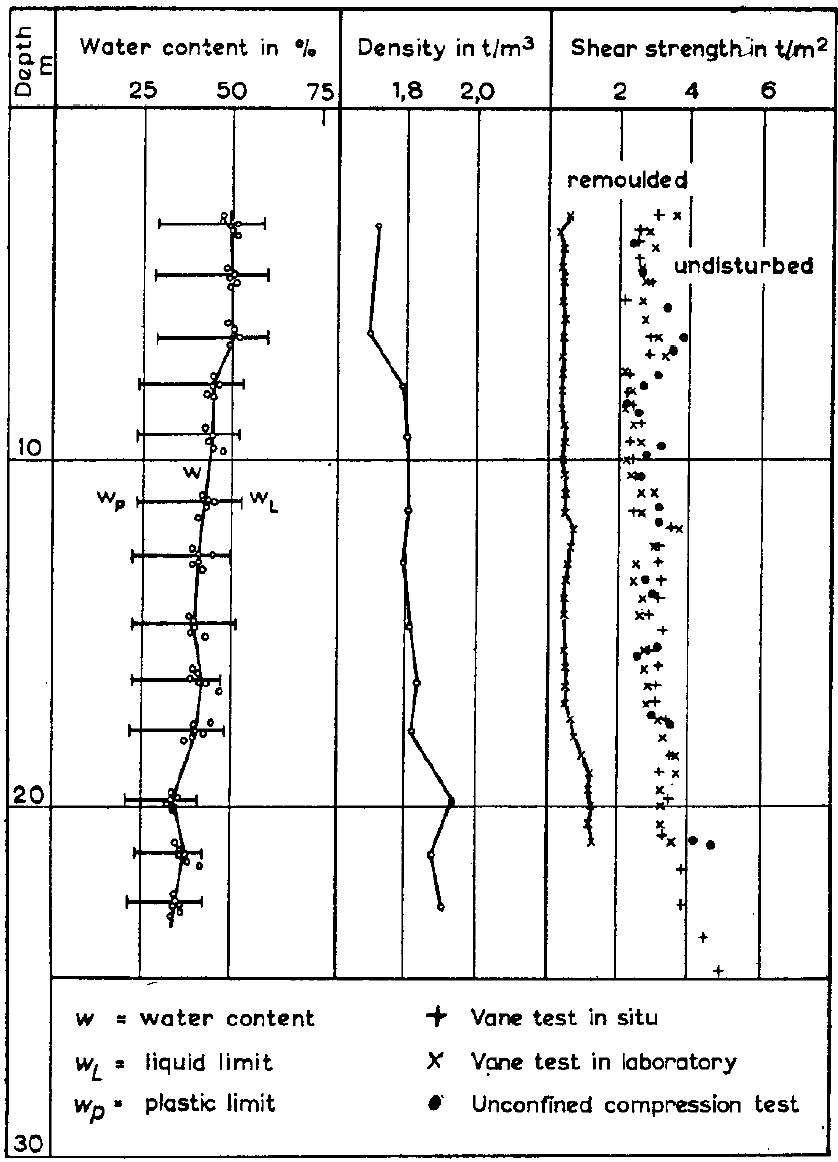
\includegraphics[width=0.5\textwidth]{figures/figure-1.png}
    \caption{Geotechnical profile through Skabo clay with results of field and laboratory tests}
    \addtocounter{figure}{-1}
    \vspace{-5pt}
    \renewcommand{\figurename}{图}
    \caption{通过Skabo黏土进行的岩土工程剖面以及现场和实验室试验的结果}
    \renewcommand{\figurename}{Figure}
    \label{figure:1}
\end{figure}


\begin{paracol}{2}

    \noindent From the boring records in \autoref{figure:1} it is seen directly that the clay, is unusually homogeneous with approximately constant Atterberg limits and water content between the depths of 8 and 18 m. 

    \switchcolumn

    \noindent 从\cnfigureref{figure:1}的记录中可以直接看到,黏土异常均匀,具有近似恒定的阿特伯格极限,并且水深在8至18 m之间。

    \switchcolumn*

    Results of X-ray examination and differential thermal analysis showed that the clay fraction was composed of about 40$\%$ illite, 20$\%$ chlorite, 25$\%$ quartz, and 15$\%$ feldspar. Except for the presence of the appreciable amount of chlorite, the mineralogical composition may be considered as typically representative of the clay in the Oslo region.

    \switchcolumn

    X射线检查和差热分析的结果表明,黏土部分由约40$\%$的伊利石,20$\%$的绿泥石,25$\%$的石英和15$\%$的长石组成。 除了存在可观数量的亚氯酸盐外,矿物​​学组成通常被认为是奥斯陆地区黏土的典型代表。

    \switchcolumn*

    The results of about forty consolidation tests showed that the soil has a "weathered" zone approximately 11 m thick and below this depth the deposit is normally consolidated. This finding is confirmed by a study of the variation in undrained shear strength with depth. Below a depth of about 11 m the clay exhibits a linear increase of shear strength with depth. The ratio of the undrained shear strength to the consolidation pressure is 0·25 for the layer considered. The undrained shear strength being determined in situ by vane tests and in the laboratory by vane tests and unconfined compression tests.

    \switchcolumn
        
    大约四十次固结试验的结果表明,土壤具有大约11 m厚的“风化”区,在该深度以下,沉积物通常被固结。 通过研究不排水抗剪强度随深度的变化,证实了这一发现。 在约11 m的深度以下,黏土的剪切强度随深度呈线性增加。 对于所考虑的层,不排水的剪切强度与固结压力之比为0.25。 不排水的剪切强度是通过现场十字板剪切试验确定的,而在实验室中是通过十字板剪切试验和无侧限压缩试验确定的。

    \switchcolumn*

    All samples tested were undisturbed but reconsolidated at a pressure well above the effect stresses which the samples carried in the field, so that they can be considered as normally consolidated.

    \switchcolumn
        
    所有试验的样品均未受干扰,但在远高于样品在野外所承受的作用应力的压力下重新固结,因此可以将其视为正常固结。
    
\end{paracol}
\section{Testing Procedure 试验程序}

\begin{paracol}{2}
    
    The tests were carried out with the triaxial equipment developed at the Norwegian Geotechnical Institute. The samples had a diameter of 3.56 cm (10 sq. cm area) and their height was 8 cm. In all tests double membranes separated with a thin layer of silicon grease were used.

    \switchcolumn

    试验是使用挪威岩土工程学院开发的三轴设备进行的。 样品的直径为3.56厘米(面积为10平方厘米),高度为8厘米。 在所有试验中,均使用用硅脂薄层隔开的双膜。

    \switchcolumn*

    In order to ensure that the samples tested were normally consolidated, the consolidation pressure used was 2.5 $\rm{kg/cm^2}$. Six samples were consolidated isotropically at this pressure and six samples were consolidated anisotropically at the major and minor principal stresses of 2.5 $\rm{kg/cm^2}$ and 1.5 $\rm{kg/cm^2}$, respectively. For each series two samples were left at the consolidation pressure for a period of 3 days, two samples for 2 weeks and the last two samples for a period of 4 months.
        
    \switchcolumn
    
    为了确保试验的样品正常固结,固结压力为2.5$\rm{kg/cm^2}$。 在该压力下六个样品进行了各向同性固结,在主应力和次主应力为2.5$\rm{kg/cm^2}$和1.5$\rm{kg/cm^2}$时,六个样品进行了各向异性固结。对于每个系列,将两个样品在固结压力下放置3天,两个样品放置2周,最后两个样品放置4个月。

    \switchcolumn*

    After these periods of aging the samples were subjected to a conventional undrained shear test with measurements of pore pressures. The shear tests were carried out with a back pressure of 2 $\rm{kg/cm^2}$ to ensure saturation, the cell pressure and the pore pressure being raised simultaneously. The strain rate used for the shear test was 1$\%$ in 48 min.

    \switchcolumn

    在进行了这些时间的固结之后,对样品进行常规的不排水剪切试验,其测量孔隙压力。 剪切试验是在2$\rm{kg/cm^2}$的背压下进行的,以确保饱和,同时提高毛细压力和孔隙压力。 用于剪切试验的应变率在48分钟内为1$\%$。

\end{paracol}
\section{Discussion Of Test Results 讨论试验结果}

\begin{sidewaystable*}[!p]
    \centering
    \caption{Results of aging tests on Skabo clay}
    \addtocounter{table}{-1}
    \vspace{-12pt}
    \renewcommand{\tablename}{表}
    \caption{Skabo黏土的时效试验结果}
    \vspace{-8pt}
    \renewcommand{\tablename}{Table}
    \tabcolsep=0.8mm
    \begin{tabularx}{\textwidth}{lllXXllllllllllllll}
        \toprule
        \multirowcell{2}[-20pt][l]{Depth:\\m} & \multirow{2}*[-25pt]{Type} & \multirowcell{2}[-20pt][l]{Time of\\consolidation} & \multicolumn{2}{l}{\makecell[l]{Consolidation\\pressure: $\rm{kg/cm^2}$}} &  &  & \multicolumn{6}{l}{$(\sigma_1-\sigma_3)_{\max}$} & \multicolumn{6}{l}{$(\sigma_1'/\sigma_3')_{\max}$} \\\cmidrule(lr){4-5}\cmidrule(lr){8-13}\cmidrule(lr){14-19}
         & & & $\sigma_1$ & $\sigma_3$ & $w_i:\%$ & $w_f:\%$ & $\varepsilon_f:\%$ & \makecell[l]{($\sigma_1-\sigma_3$):\\$\rm{kg/cm^2}$} & \makecell[l]{$\Delta{u}$:\\$\rm{kg/cm^2}$} & $A$ & $\sigma_1'/\sigma_3'$ & \makecell[l]{Time to\\failure: min} & $\varepsilon:\%$ & \makecell[l]{($\sigma_1-\sigma_3$):\\$\rm{kg/cm^2}$} & \makecell[l]{$\Delta{u}$:\\$\rm{kg/cm^2}$} & $A$ & $\sigma_1'\sigma_3'$ & \makecell[l]{Time to\\failure: min}\\
        \midrule
        15.10  & CIU   & 3 days & 2.5   & 2.5   & 41.6  & 33.1  & 3.8   & 1.75  & 1.63  & 0.93  & 3.02  & 200   & 8.3   & 1.74  & 1.81  & 1.04  & 3.53  & 404 \\     15.45  & CIU   & 4 days & 2.5   & 2.5   & 48.2  & 38.2  & 3.3   & 1.70  & 1.59  & 0.94  & 2.87  & 223   & 8.4   & 1.67  & 1.82  & 1.09  & 3.45  & 448 \\     15.75  & CAU   & 5 days & 2.5   & 1.5   & 39.4  & 34.4  & 1.9   & 1.76  & 0.59  & 0.78  & 2.94  & 335   & 9.4   & 1.66  & 0.77  & 1.16  & 3.28  & 1128 \\     15.85  & CAU   & 6 days & 2.5   & 1.5   & 40.0  & 33.4  & 2.3   & 1.78  & 0.72  & 0.93  & 3.28  & 307   & 10.6  & 1.68  & 0.90  & 1.33  & 3.79  & 1255 \\     15.40  & CIU   & 2 weeks & 2.5   & 2.5   & 40.6  & 32.7  & 3.6   & 1.89  & 1.57  & 0.83  & 3.04  & 195   & 11.8  & 1.90  & 1.77  & 0.93  & 3.60  & 571 \\     15.50  & CIU   & 3 weeks & 2.5   & 2.5   & 41.2  & 32.4  & 4.3   & 1.90  & 1.63  & 0.86  & 3.18  & 230   & 9.3   & 1.85  & 1.72  & 0.93  & 3.37  & 456 \\     15.75  & CAU   & 4 weeks & 2.5   & 1.5   & 42.8  & 33.4  & 0.9   & 1.90  & 0.47  & 0.52  & 2.85  & 135   & 5.0   & 1.76  & 0.77  & 1.01  & 3.41  & 635 \\     15.85  & CAU   & 5 weeks & 2.5   & 1.5   & 43.2  & 33.5  & 0.8   & 1.78  & 0.48  & 0.62  & 2.74  & 124   & 11.8  & 1.46  & 1.00  & 2.17  & 3.93  & 1382 \\     15.35  & CIU   & 4 months & 2.5   & 2.5   & 47.8  & 37.6  & 2.0   & 1.85  & 1.31  & 0.71  & 2.55  & 116   & 10.1  & 1.65  & 1.80  & 1.09  & 3.36  & 452 \\     15.55  & CIU   & 5 months & 2.5   & 2.5   & 46.5  & 36.4  & 2.2   & 1.97  & 1.40  & 0.71  & 2.78  & 135   & 8.9   & 1.77  & 1.79  & 1.02  & 3.49  & 435 \\     16.10  & CAU   & 6 months & 2.5   & 1.5   & 41.9  & 35.4  & 0.5   & 1.74  & 0.36  & 0.49  & 2.53  & 99    & 12.0  & 1.32  & 0.91  & 2.84  & 3.24  & 1481 \\     16.20  & CAU   & 7 months & 2.5   & 1.5   & 43.5  & 36.2  & 0.5   & 2.02  & 0.34  & 0.34  & 2.74  & 100   & 11.0  & 1.54  & 0.92  & 1.70  & 3.66  & 1270 \\ 
        \bottomrule
    \end{tabularx}%
    \label{table:2}%
    \vspace{10pt}
    \caption{Results of aging tests on Skabo clay}
    \addtocounter{table}{-1}
    \vspace{-12pt}
    \renewcommand{\tablename}{表}
    \caption{Skabo黏土的时效试验结果}
    \vspace{-8pt}
    \renewcommand{\tablename}{Table}
    \begin{tabularx}{\textwidth}{llXXXXXXXXXXXXl}
        \toprule
        \multirowcell{2}[-6pt][l]{Type of\\test:} & \multirowcell{2}[-6pt][l]{Time of \\consolidation} & \multicolumn{2}{l}{Water content:} & \multicolumn{6}{l}{At $(\sigma_1-\sigma_3)_{\max}$} & \multicolumn{5}{l}{At $(\sigma_1'/\sigma_3')_{\max}$} \\\cmidrule(lr){3-4}\cmidrule(lr){5-10}\cmidrule(lr){11-15}
         & & $w_i$ & $w_f$ & $\varepsilon:\%$ & $\frac{(\sigma_1-\sigma_3)/2}{p}$ & $\sigma_1'/\sigma_3'$ & $\phi'$ & $D_M:\%$ & $A_f$ & $\varepsilon:\%$ & $\sigma_1'/\sigma_3'$ & $\phi'_u$ & $A$ & $\frac{\Delta{u}}{p}+1-K$ \\
         \midrule
         CIU & \makecell[l]{3 days\\2 weeks\\4 months} & \makecell[l]{44.9\\40.9\\37.0} & \makecell[l]{35.7\\32.5\\37.0} & \makecell[l]{3.6\\4.0\\2.1} & \makecell[l]{0.346\\0.379\\0.382} & \makecell[l]{2.95\\3.12\\2.67} & \makecell[l]{29.6°\\31.0°\\27.0°} & \makecell[l]{85\\90\\78} & \makecell[l]{0.94\\0.85\\0.71} & \makecell[l]{~8.4\\10.6\\~9.5} & \makecell[l]{3.49\\3.49\\3.43} & \makecell[l]{33.7°\\33.7°\\33.2°} & \makecell[l]{1.07\\0.93\\1.05} & \makecell[l]{0.72\\0.70\\0.72}\\
         CAU & \makecell[l]{3 days\\2 weeks\\4 months} & \makecell[l]{39.7\\43.0\\42.7} & \makecell[l]{33.9\\33.4\\35.8} & \makecell[l]{2.1\\0.9\\0.5} & \makecell[l]{0.354\\0.368\\0.376} & \makecell[l]{3.11\\2.80\\2.64} & \makecell[l]{30.8°\\28.3°\\26.8°} & \makecell[l]{88\\85\\77} & \makecell[l]{0.88\\0.57\\0.42} & \makecell[l]{10.0\\~8.4\\11.5} & \makecell[l]{3.54\\3.67\\3.45} & \makecell[l]{34.0°\\33.9°\\33.4} & \makecell[l]{1.24\\1.59\\2.27} & \makecell[l]{0.73\\0.75\\0.77} \\
        \bottomrule
    \end{tabularx}
    \label{table:3}
\end{sidewaystable*}


\begin{paracol}{2}
    
    Since all tests were performed in duplicate and because samples consolidated isotropically as well as anisotropically were allowed to age for three different periods, the test series includes in total twelve tests. The details of the test results are collected in \autoref{table:2} and some of the most important characteristics are summarized in \autoref{table:3}.

    \switchcolumn

    由于所有试验均一式两份进行,并且由于各向同性和各向异性固结的样品可以老化三个不同的时期,因此试验系列总共包括十二个试验。 \cntableref{table:2}收集了试验结果的详细信息,\cntableref{table:3}总结了一些最重要的特性。

    \switchcolumn*

    In \autoref{table:2} the failure parameters are listed, whereby it has been distinguished between the bulk failure of the sample at the peak value of the principal stress difference $(\sigma_1-\sigma_3)_{\max}$ and the ultimate failure of the soil skeleton occurring at maximum effective principal stress ratio $(\sigma_1'/\sigma_3')_{\max}$.

    \switchcolumn
       
    在\cntableref{table:2}中列出了破坏参数,从而区分了在主应力差$(\sigma_1-\sigma_3)_{\max}$峰值处的样品整体破坏和在最大有效主应力比$(\sigma_1'/\sigma_3')_{\max}$下发生的土体骨架的最终破坏。
    
    \switchcolumn*

    Before discussing the effect of the age on the shear strength characteristics, it is of importance to realize that there was no appreciable reduction in water content of the samples during the aging periods. This observation is confirmed by the measurements of the final water contents, see \autoref{table:3}, which do not show any regular decrease with the period of aging.

    \switchcolumn

    在讨论时效对剪切强度特性的影响之前,重要的是要认识到,时效期间样品的含水量没有明显降低。 最终水含量的测量结果证实了这一观察结果,请参见\cntableref{table:3},\cntableref{table:3}没有显示出随时间的任何规律性下降。

    \switchcolumn*

    From the shear-strength characteristics computed at the peak values of $(\sigma_1-\sigma_3)$ and $\sigma_1'/\sigma_3'$ and listed in \autoref{table:2} and \autoref{table:3} the following conclusions can be drawn: 

    \switchcolumn
       
    根据在$(\sigma_1-\sigma_3)$和$\sigma_1'/\sigma_3'$的峰值处计算并在\cntableref{table:2}和\cntableref{table:3}中列出的抗剪强度特性,可以得出以下结论:
     
    \switchcolumn*
    
    \noindent \emph{At $(\sigma_1-\sigma_3)_{\max}$ the effect of an increase of period of aging is:}
    
    ($a$) the undrained shear strengt $\dfrac{1}{2}(\sigma_1-\sigma_3)/p$ increase slightly; 

    ($b$) the pore-pressure parameter $A_f$ decreases; 

    ($c$) the strain at failure decreases; 

    ($d$) the angle of shearing resistance$\phi'$ mobilized at $(\sigma_1-\sigma_3)_{\max}$ decreases and the degree of mobilization defined as: $D_M=\tan\phi'/\tan\phi'_u$ thus decreases.

    \noindent \emph{At $(\sigma_1'-\sigma_3')_{\max}$ the effect is:}

    ($e$) the maximum principal effective stress ratio $\sigma_1'-\sigma_3'$ remains unchanged and so does the ultimate angle of shearing resistance $\phi'_u$;

    ($f$) the pore-pressure parameter A remains unchanged for the samples consolidated isotropically, but increases for the anisotropically consolidated samples.

    \switchcolumn

    \noindent \emph{在$(\sigma_1-\sigma_3)_{\max}$处,时间增加的影响为:}

    ($a$) 不排水的剪切强度$\dfrac{1}{2}(\sigma_1-\sigma_3)/p$略有增加;  

    ($b$) 孔隙压力参数$A_f$减小;  

    ($c$) 破坏应变降低;

    ($d$) 在$(\sigma_1-\sigma_3)_{\max}$处调动的抗剪角$\phi'$减小,将调动程度定义为:$D_M=\tan\phi'/\tan\phi'_u$,因此也相应减小。

    \noindent \emph{在$(\sigma_1'-\sigma_3')_{\max}$处,影响为为:}

   ($e$) 最大主有效应力比$\sigma_1'-\sigma_3'$保持不变,抗剪极限角$\phi'_u$也保持不变;

   ($f$) 对于各向同性固结的样品,孔隙压力参数$A$保持不变,但对于各向异性固结的样品,参数$A$则增加。

   \switchcolumn*

   The conclusions drawn may well be useful for an evaluation of the effect of time on the conventionally used shear strength parameters, but they contribute only little to a fundamental understanding of the change of properties of a clay occurring when it is left at a sustained consolidation pressure for a period of time. Much can however be learned from a study of the stress-strain properties and for this purpose the test results have been plotted in \autoref{figure:2} and \autoref{figure:3}. For a comparison of the stress-strain properties of a number of tests it has previously been found convenient to make use of the following equation which is generally valid and holds good for any strain :

   \switchcolumn

   得出的结论可能对评估时间对常规使用的剪切强度参数的影响很有用,但对于基本了解黏土保持一段时间持续固结压力时所发生的特性变化的作用不大。然而,从应力-应变特性的研究中可以学到很多,为此目的,试验结果绘制在\cnfigureref{figure:2}和\cnfigureref{figure:3}中。为了比较许多试验的应力-应变特性,以前发现很方便利用以下等式,该等式通常有效,并且对任何应变都适用: 

\end{paracol}

\begin{align}
    \frac{\sigma_1-\sigma_3}{p}=(\sigma_1'/\sigma_3'-1)\left[1-\left(\frac{\Delta{u}}{p}+(1-K)\right)\right]
\end{align}
\begin{figure*}
    \begin{minipage}[t]{0.51\textwidth}
        \centering
        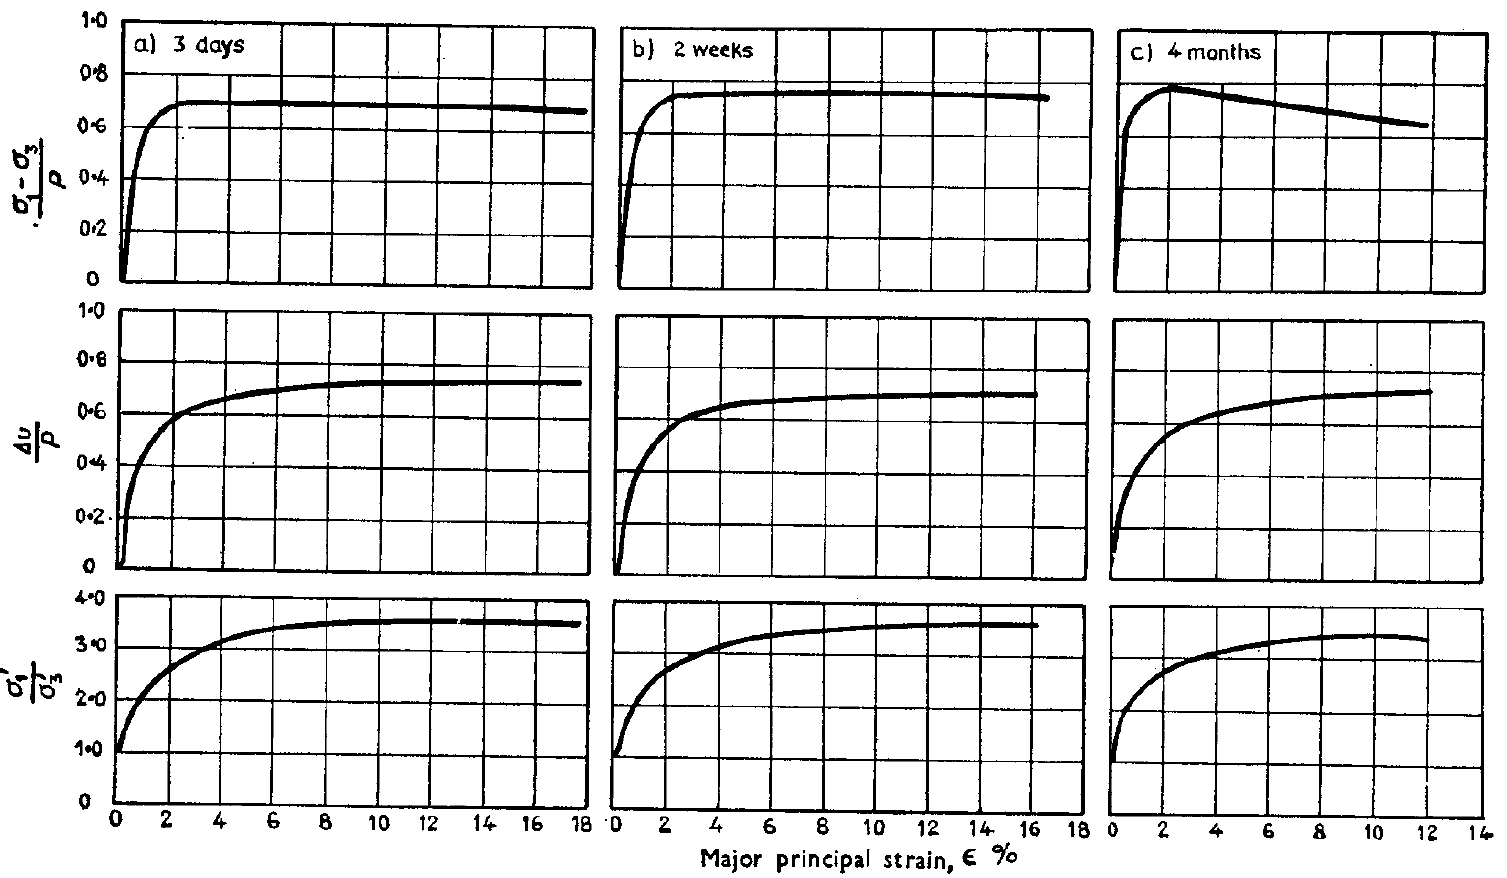
\includegraphics[width=\textwidth]{figures/figure-2.png}
        \caption{Results of consolidated undrained triaxial tests on samples consolidated isotropically for various periods of times: (a) 3 days, (b) 2 weeks, (c) 4 months. Consolidation pressure 25 $\rm{kg/sq\cdot{cm}}$. Each curve represents the average of two tests.}
        \addtocounter{figure}{-1}
        \vspace{-5pt}
        \renewcommand{\figurename}{图}
        \caption{各向同性固结样品在不同时间段的固结不排水三轴试验结果:(a)3天,(b)2周,(c)4个月。 固结压力25$\rm{kg/sq\cdot{cm}}$。 每条曲线代表两次试验的平均值。}
        \renewcommand{\figurename}{Figure}
        \label{figure:2}
    \end{minipage}
    \begin{minipage}[t]{0.44\textwidth}
        \centering
        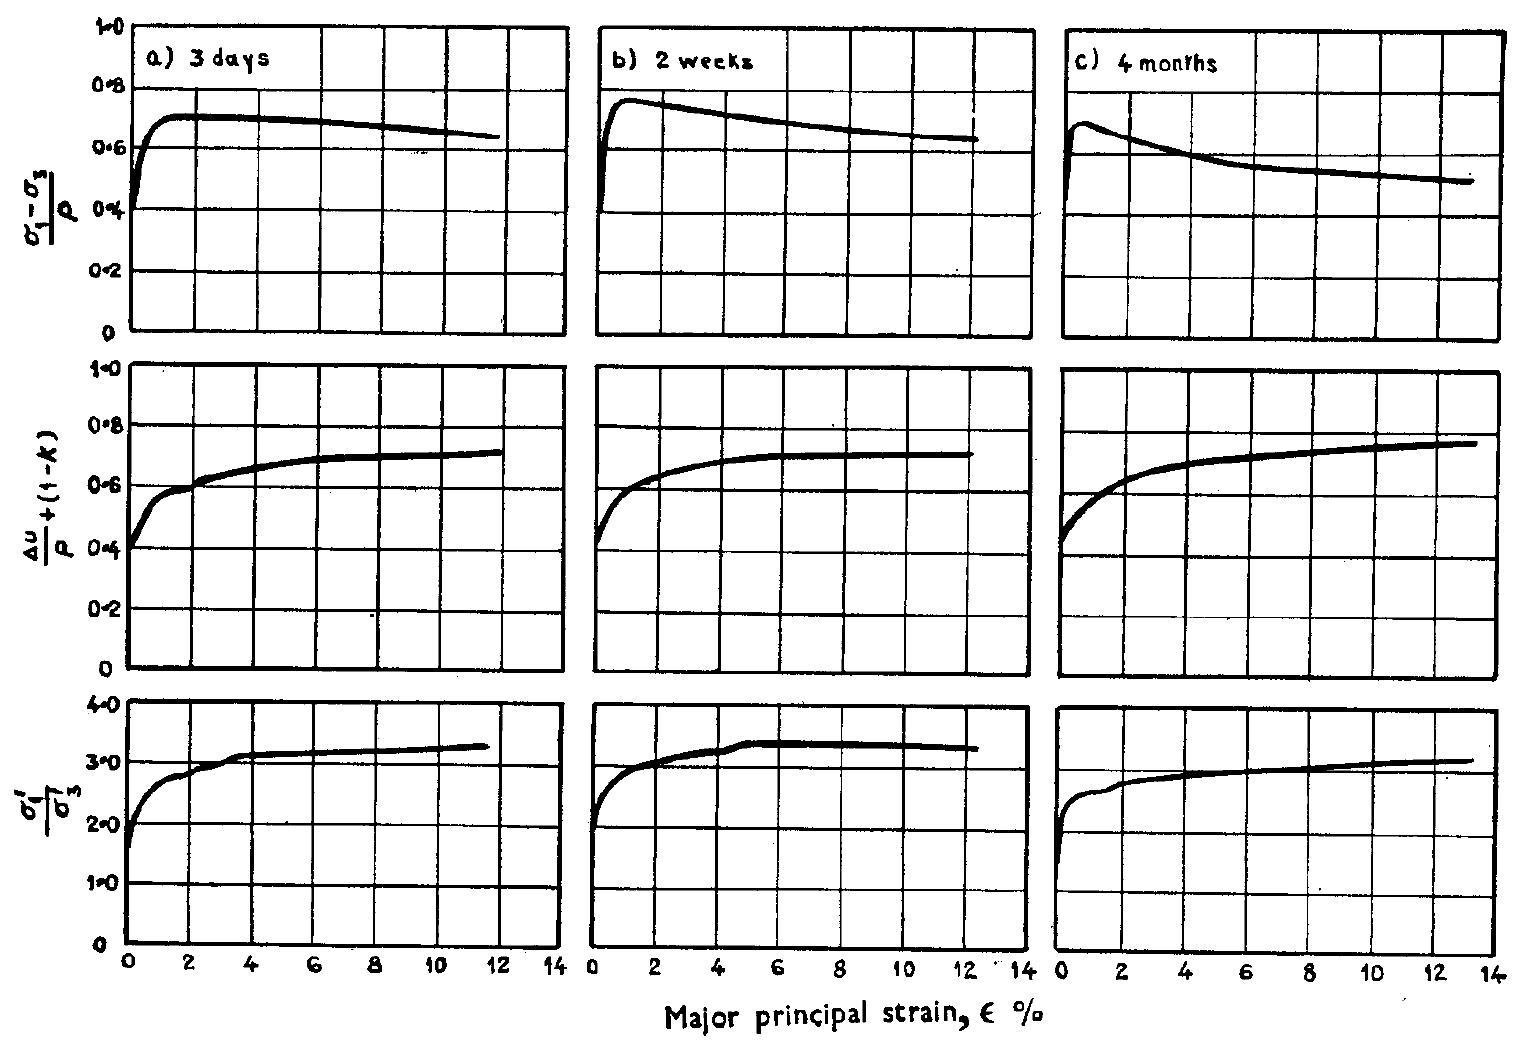
\includegraphics[width=\textwidth]{figures/figure-3.png}
        \caption{Results of consolidated undrained triaxial tests on samples consolidated anisotropically for various periods of times: (a) 3 days, (b) 2 weeks, (c) 4 months.
        Consolidation pressure $p_1=2.5\rm{kg/sq\cdot{cm}},p_2=p_3=1.5\rm{kg/sq\cdot{cm}}$. Each curve represents the average of two tests}
        \addtocounter{figure}{-1}
        \vspace{-5pt}
        \renewcommand{\figurename}{图}
        \caption{在不同时间段进行各向异性固结的样品的固结不排水三轴试验结果:(a)3天,(b)2周,(c)4个月。固结压力$p_1=2.5\rm{kg/sq\cdot{cm}},p_2=p_3=1.5\rm{kg/sq\cdot{cm}}$。每条曲线代表两次试验的平均值}
        \renewcommand{\figurename}{Figure}
        \label{figure:3}
    \end{minipage}
\end{figure*}

\begin{paracol}{2}
    
    \noindent in which $p$ and $Kp$ represent the major and minor principal consolidation pressures. In this equation $\sigma_1'/\sigma_3'-1$ and $\Delta{u}/p$ are considered to be independent functions of the strain and these functions will be discussed separately.

    \switchcolumn

    \noindent 式中$p$和$Kp$代表主要和次要固结应力。在该方程中,$\sigma_1'/\sigma_3'-1$和$\Delta{u}/p$被认为是应变的独立函数,并且将分别讨论这些函数。

\end{paracol}
\section{Effect Of Aging On $\dfrac{\Delta{u}}{p}-\varepsilon$ Relationship 时效对$\dfrac{\Delta{u}}{p}-\varepsilon$关系的影响}

\begin{paracol}{2}
    
    The change of pore-pressure ratio $\Delta{u}/p$ in relation to strain for all the samples consolidated isotropically and anisotropically are plotted in \autoref{figure:4a} and \autoref{figure:4b}, respectively.

    \switchcolumn

    对于各向同性和各向异性固结的所有样品,孔隙压力比$\Delta{u}/p$随应变的变化分别绘制在\cnsubfigureref{figure:4a}和\cnsubfigureref{figure:4b}中。

    \switchcolumn*

    \autoref{figure:4a} shows clearly that in spite of the different period of aging a unique relationship exists between excess pore-pressure and major principal strain. The points resulting from the performed six tests on the isotropically consolidated samples fall very close to a single curve. The conclusion may therefore be reached that aging has no effect on the porepressure/strain relationship.

    \switchcolumn
        
    \cnsubfigureref{figure:4a}清楚地表明,尽管老化时间不同,但在超孔隙压力和主要主应变之间仍存在独特的关系。 对各向同性固结样品进行六次试验所得的点非常接近一条曲线。 因此可以得出结论,时效对孔压/应变关系没有影响。

    \switchcolumn*

    \autoref{figure:4b} are plotted the excess pore pressures observed during the shearing of the anisotropically consolidated samples. These test results show a considerable scatter, but a detailed study shows that the variation of the observed pore pressures does not correspond to or is not correlated with any specific variable such as time of aging or the water content. It is believed, therefore, that the scatter is a result of small variations of principal stress ratio during the consolidation \citep{Lo1961219}.

    \switchcolumn
        
    在\cnsubfigureref{figure:4b}中,绘制了在各向异性固结样品剪切过程中观察到的多余孔隙压力。 这些试验结果显示出相当大的分散性,但是详细的研究表明,观察到的孔隙压力的变化与任何特定变量(例如老化时间或含水量)不对应或不相关。 因此,可以认为,分散是固结过程中主应力比的微小变化的结果\citep{Lo1961219}。

\end{paracol}

\begin{figure}[!htbp]
    \centering
    \subfigure[CIU, tests on isotropically consolidated samples]{
        \label{figure:4a}
        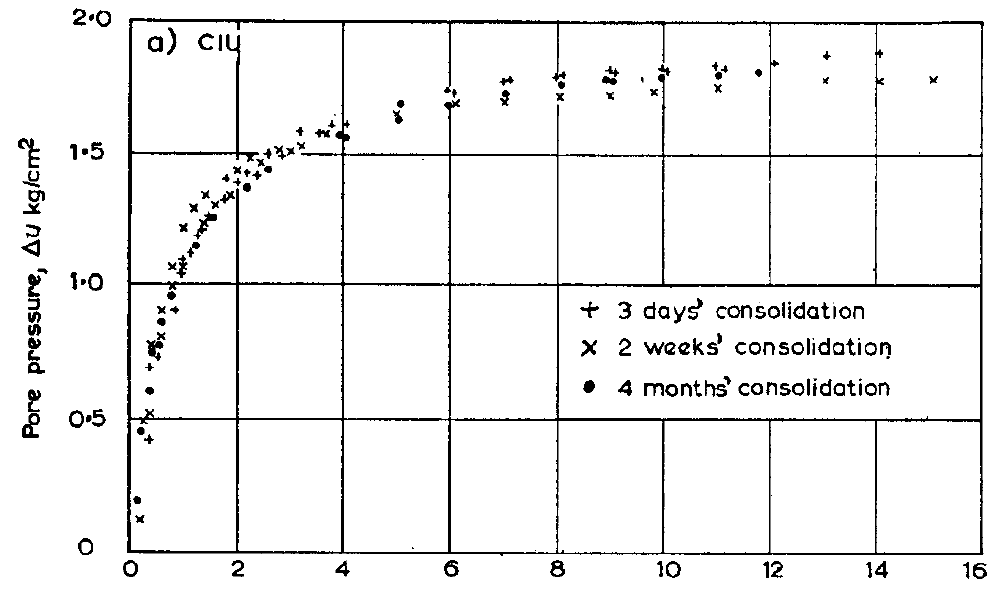
\includegraphics[width=0.43\textwidth]{figures/figure-4a.png}
    }
    \subfigure[CAU, tests on anisotropically consolidated samples]{
        \label{figure:4b}
        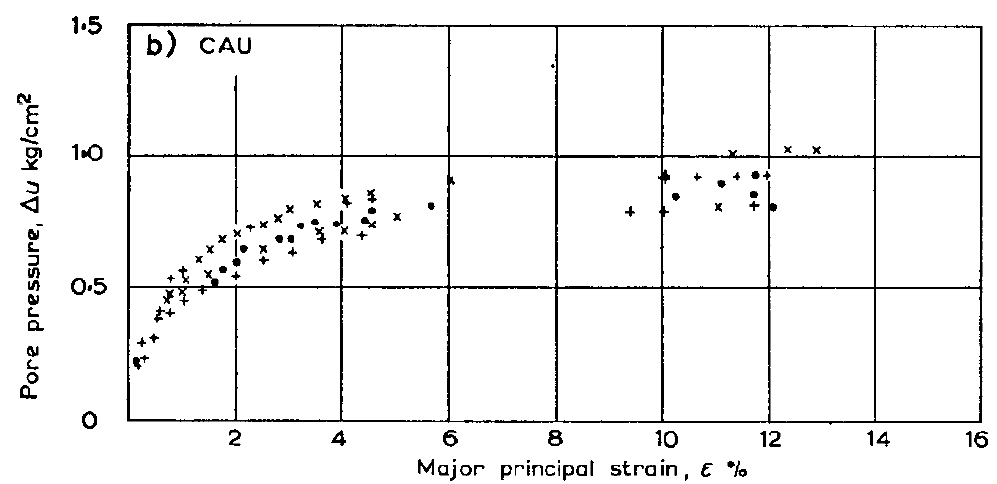
\includegraphics[width=0.53\textwidth]{figures/figure-4b.png}
    }
    \caption{Excess pore pressure set up during consolidated undrained tests, For each type of consolidation are shown the results of six separate tests.}
    \addtocounter{figure}{-1}
    \vspace{-5pt}
    \renewcommand{\figurename}{图}
    \caption{在固结不排水的综合试验中设置了过多的孔隙压力,对于每种类型的固结试验,均显示六个独立试验的结果。}
    \renewcommand{\figurename}{Figure}
    \label{figure:4}
\end{figure}

\begin{paracol}{2}
    

    The maximum values of $\Delta{u}/p+(1-K)$ are listed in \autoref{table:3} for comparison. The values determined for the anisotropically consolidated samples are slightly higher than those observed for the isotropical samples, a finding which has been confirmed also for other types of clay \citep{Bjerrum196123b}. The tests on the isotropical samples show no tendency for this quantity to vary with the time of aging, but a small increase with time of aging was observed for the samples consolidated anisotropically.

    \switchcolumn

    \cntableref{table:3}中列出了$\Delta{u}/p+(1-K)$的最大值以进行比较。 各向异性固结样品的测定值略高于各向同性样品的观察值,这一发现在其他类型的黏土中也得到了证实\citep{Bjerrum196123b}。在各向同性样品上进行的试验表明,该数量没有随老化时间变化的趋势,但对于各向异性固结的样品,随老化时间的增加却很小。

\end{paracol}
\section{Effect Of Aging On $\sigma_1'/\sigma_3'-\varepsilon$ Relationship 时效对$\sigma_1'/\sigma_3'-\varepsilon$关系的影响}

\begin{paracol}{2}
    
    In \autoref{figure:5a} and \autoref{figure:5b} are shown the variation of principal effective stress ratio with strain for samples consolidated isotropically and anisotropically, respectively.

    \switchcolumn

    在\cnsubfigureref{figure:5a}和\cnsubfigureref{figure:5b}中分别示出了各向同性和各向异性固结的样品的主要有效应力比随应变的变化。

    \switchcolumn*

    From the plotted curves it is observed at once that at a given strain the effective principal stress ratio is higher for samples with longer period of consolidation. However, the curves converge into a single one as the ratios approach their maximum value. This trend is observed for both the isotropically and the anisotropically consolidated samples, with the exception that the curve for samples consolidated anisotropically over a period of 4 months lies below the two others for large strains.

    \switchcolumn
       
    从绘制的曲线可以立即观察到,在给定应变下,固结时间较长的样品的有效主应力比较高。 但是,随着比率接近其最大值,曲线会收敛为一条曲线。 对于各向同性和各向异性固结的样品,都观察到了这种趋势,不同的是,在四个月的时间内,各向异性固结的样品的曲线低于大应变的两个曲线。

    \switchcolumn*

    The maximum values of $\sigma_1'/\sigma_3'$ are listed in \autoref{table:3} and they show no pronounced variation with the period of aging; if anything, there is a tendency towards a small reduction with aging.

    \switchcolumn
       
    \cntableref{table:3}中列出了$\sigma_1'/\sigma_3'$的最大值,并且它们没有显示出随老化时间的明显变化。 如果有的话,随着时间的流逝有减少的趋势。

\end{paracol}

\begin{figure}[!htbp]
    \centering
    \subfigure[CIU, tests on isotropically consolidated samples]{
        \label{figure:5a}
        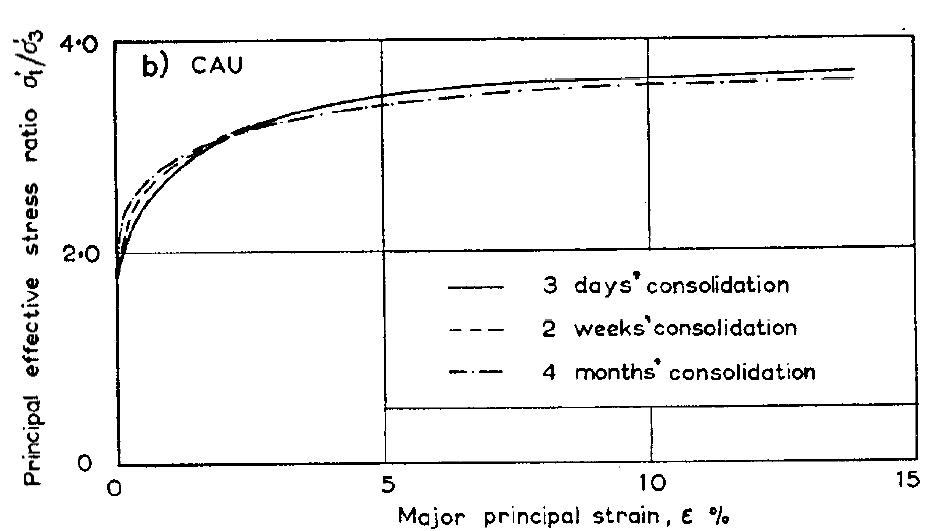
\includegraphics[width=0.48\textwidth]{figures/figure-5a.png}
    }
    \subfigure[CAU, tests on anisotropically consolidated samples]{
        \label{figure:5b}
        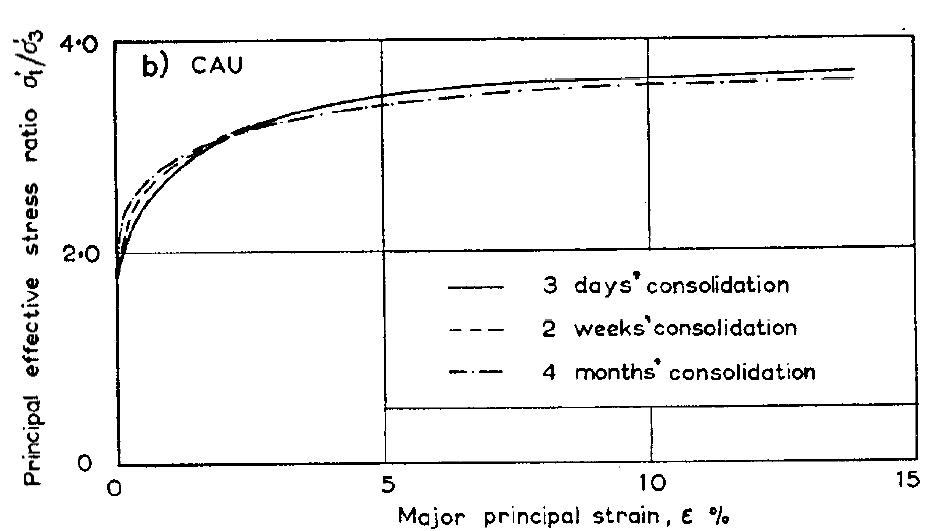
\includegraphics[width=0.48\textwidth]{figures/figure-5b.png}
    }
    \caption{Principal effective stress ratio as observed in consolidated undrained tests, Each curve represents the average of two tests.}
    \addtocounter{figure}{-1}
    \vspace{-5pt}
    \renewcommand{\figurename}{图}
    \caption{固结不排水试验中观察到的主要有效应力比,每条曲线代表两次试验的平均值。}
    \renewcommand{\figurename}{Figure}
    \label{figure:5}
\end{figure}
\section{Effect Of Aging On $\dfrac{\sigma_1-\sigma_3}{p}-\varepsilon$ Relationship \\时效对$\dfrac{\sigma_1-\sigma_3}{p}-\varepsilon$关系的影响}

\begin{paracol}{2}
    
    From the graphical plots of the test results in \autoref{figure:2} and \autoref{figure:3} it is directly seen that an aging has a very marked influence on the $(\sigma_1-\sigma_3)$ — strain relationship. For an increased period of aging the maximum value of $\sigma_1-\sigma_3$ occurs at a smaller strain and the reduction in $\sigma_1-\sigma_3$ after failure becomes more pronounced.

    \switchcolumn

    从\cnfigureref{figure:2}和\cnfigureref{figure:3}的试验结果的图形图中可以直接看出,时效对$(\sigma_1-\sigma_3)$-应变关系具有非常显着的影响。 随着老化时间的延长,$\sigma_1-\sigma_3$的最大值出现在较小的应变下,而失效后$\sigma_1-\sigma_3$的减小变得更加明显。

    \switchcolumn*

    Considering the maximum values of $\sigma_1-\sigma_3$ there is a slight increase in the undrained compressive strength of the samples with aging. This increase is of the order of $6-10\%$ for the range of time variations investigated in the present test series.

    \switchcolumn
       
    考虑到$\sigma_1-\sigma_3$的最大值,样品的不排水抗压强度会随着老化而略有增加。 对于本试验系列中研究的时间变化范围,这种增加约为$6-10\%$。

    \switchcolumn*

    Now, the value of a1 $(\sigma_1-\sigma_3)/p$ is at any strain a function of the two basic parameters $\Delta{u}/p$ and $\sigma_1'/\sigma_3'$ as expressed by the equation:

    \switchcolumn
       
    现在,在任何应变下,$(\sigma_1-\sigma_3)/p$的值都是两个基本参数$\Delta{u}/p$和$\sigma_1'/\sigma_3'$的函数,如方程式所示: 

\end{paracol}

\begin{align}
    \dfrac{\sigma_1-\sigma_3}{p}=(\sigma_1'/\sigma_3'-1)\left\{1-\left[\frac{\Delta{u}}{p}+(1-K)\right]\right\}
\end{align}

\begin{paracol}{2}

    $(\sigma_1-\sigma_3)/p$ is thus a product of a "strength term" $(\sigma_1'/\sigma_3'-1)$ which increases with strain and an "effective stress term" $ \left\{1-\left[\frac{\Delta{u}}{p}+(1-K)\right]\right\}$ which in undramed tests on normally consolidated clays decreases for increasing strain. The maximum value of $(\sigma_1-\sigma_3)/p$ will, therefore, in general not occur at the strain where the stren?th term is maximum, but at an intermediate strain where the rate of decrease of the effective stress term just compensates the rate of increase of the strength term, i.e. when:

    \switchcolumn

    因此,$(\sigma_1-\sigma_3)/p$是“强度项”$(\sigma_1'/\sigma_3'-1)$的乘积项,该强度项随应变而增加,而“有效应力项”$ \left\{1-\left[\frac{\Delta{u}}{p}+(1-K)\right]\right\}$在正常固结的黏土上,随应变的增加而减少。 因此,$(\sigma_1-\sigma_3)/p$的最大值通常不会出现在强度项最大的应变处,而出现在中间应变处,有效应力项的减小率只会补偿强度的增加率,例如,当下述条件满足时:

\end{paracol}

\begin{align}
    \frac{\dfrac{d\left(\dfrac{\Delta{u}}{p}\right)}{d\varepsilon}}{1-\left[\dfrac{\Delta{u}}{p}+(1-K)\right]}=\frac{\dfrac{d(\sigma_1'/\sigma_3')}{d\varepsilon}}{\sigma_1'/\sigma_3'-1}
\end{align}

\begin{paracol}{2}

    This fact explains the observation from tests on normally consolidated clays that there is a rise in pore pressure at the peak value of $\sigma_1-\sigma_3$.

    \switchcolumn

    这一事实解释了从对正常固结黏土的试验中观察到的结果,即在$\sigma_1-\sigma_3$的峰值处,孔隙压力有所增加。

    \switchcolumn*

    Turning the attention towards the effect of aging, it has been shown above that the $\Delta{u}/p-\varepsilon$ relationship does not change with aging, whereas the $\sigma_1'/\sigma_3'-\varepsilon$ curves show a steeper rise at small strains. Consequently, the $(\sigma_1-\sigma_3)-\varepsilon$ curves will rise more steeply and reach maximum values at smaller strains for longer aging periods. A decrease of failure strain with aging will also mean a corresponding smaller value of excess pore pressure at failure. For example, when the aging period for the CAU tests was increased from 3 days to 4 months the maximum value of $\sigma_1-\sigma_3$ changed only very little, about 6$\%$, whereas the pore pressure at failure was reduced by about 50$\%$. This explains why the A value is reduced from 0.88 to 0.41 in spite of the fact that the excess pore-pressure/strain relationship is not influenced by aging. Again, as the strain at failure decreases, the $\sigma_1'/\sigma_3'$ value at $(\sigma_1-\sigma_3)_{\max}$ is reduced, and for the samples which were consolidated for a period of 4 months the degree of mobilization at failure was as low as 77-78$\%$.

    \switchcolumn

    将注意力转移到老化的影响上,上面已经表明,$\Delta{u}/p-\varepsilon$关系不会随老化而改变,而$\sigma_1'/\sigma_3'-\varepsilon$曲线显示了在小应变下的陡峭上升。 因此,$(\sigma_1-\sigma_3)-\varepsilon$曲线将更陡峭地上升,并在较小的应变下达到更长的老化时间并达到最大值。 失效应变随老化的降低也将意味着失效时过大孔隙压力的相应较小值。 例如,当CAU试验的老化时间从3天增加到4个月时,$\sigma_1-\sigma_3$的最大值变化很小,约为6$\%$,而失效时的孔隙压力降低了约50$\%$。 这解释了为什么尽管过量的孔压/应变关系不受老化的影响,但$A$值仍从0.88降低到0.41。 同样,随着破坏应变的降低,$(\sigma_1-\sigma_3)_{\max}$处的$\sigma_1'/\sigma_3'$值也降低了,对于固结了4个月的样品,破坏时的调动程度低至77-78$\%$  。

\end{paracol}
\section{Some Notes On Development Of A Structual Stress With Time \\随着时间发展结构强度的一些注意事项}

\begin{paracol}{2}
    
    Because the samples showed initially the same structure and because the secondary consolidation was insignificant, the samples for each mode of consolidation had the same structure prior to the shear test. At a given strain it is believed that approximately the same number of contact points are broken, resulting in identical magnitudes of pore pressure set up due to transference to the pore-water of effective stresses originally carried at the contact points. To produce a given strain, a higher value of $\sigma_1'/\sigma_3'$is required for the samples consolidated 4 months than for those consolidated only 3 days. The conceivable effect of aging is therefore a growth of bond strength at the points of contact of the particles.

    \switchcolumn

    由于样品最初显示出相同的结构,并且由于次固结不明显,因此在剪切试验之前,每种固结模式的样品都具有相同的结构。 在给定的应变下,据信破裂了大约相同数量的接触点,这导致了相同大小的孔隙压力,这是由于最初在接触点处承载的有效应力转移到孔隙水中而形成的。 为了产生给定的应变,固结4个月的样品比仅固结3天的样品需要更高的$\sigma_1'/\sigma_3'$值。 因此,老化的可能效果是在颗粒接触点处粘结强度的增加。

    \switchcolumn*

    As the strain increases, movement occurs at most or all of the contact points and the bonds developed during the consolidation period are destroyed. The $\sigma_1'/\sigma_3'$ values for different aging periods therefore gradually converge into a single curve and their final maximum value is independent of the initial bond strength. The additional cohesive component of the shear strength gained with time during a consolidation period is therefore destroyed, at small strains and does not contribute to the final strength of the soil skeleton.

    \switchcolumn
    
    随着应变增加,运动最多或所有接触点发生,固结期间形成的键被破坏。因此,不同老化时期的$\sigma_1'/\sigma_3'$值逐渐收敛为一条曲线,其最终最大值与初始粘结强度无关。因此,在固结期间随时间获得的抗剪强度的附加内聚成分会在小应变下被破坏,并且不会增加土壤骨架的最终强度。

    \switchcolumn*

    It is reasonable to expect that the structure of the soil samples varies with different modes of consolidation. It is therefore also conceivable that the pore-pressure and effective stressratio characteristics might be slightly different during the early stages of the shearing process of the isotropically and the anisotropically consolidated samples. At large strains when the initial bonds have been destroyed, the mechanical behaviour of the particles is gradually dominated by sliding. It is therefore logical to expect that the ultimate values of the effective principal stress ratio would be the same for both isotropically and anisotropically consolidated samples, and this has been shown to be the case, as seen from \autoref{table:3}.

    \switchcolumn
    
    可以合理预期土壤样品的结构会随着固结模式的不同而变化。因此,还可以想象,在各向同性和各向异性固结样品的剪切过程的早期,孔隙压力和有效应力特性可能会略有不同。在较大的应变下,当初始键被破坏时,颗粒的机械行为逐渐受到滑动的支配。因此,可以合理地预期,各向同性和各向异性固结样品的有效主应力比的最终值将相同,并且从\cntableref{table:3}中可以看出情况确实如此。

    \switchcolumn*
    
    There are no reasons to believe that the bonds developed at the contact points during the 4 months of aging included in the present test programme represent the maximum values which can be reached in geological time. On the contrary, there are good reasons to believe that these bonds, which do not show up in conventional shear tests on reconsolidated samples, are of considerably greater importance in nature than observed in the tests.

    \switchcolumn
   
    没有理由相信本试验程序中包括的在老化的4个月期间在接触点处形成的键代表了在地质时间内可以达到的最大值。相反,有充分的理由相信,这些结合力在自然界比在试验中观察到的重要性要大得多,这些结合力在常规的重塑样品的剪切试验中没有表现出来。

    \switchcolumn*
    
    Even if the test results do not permit a quantitative evaluation of the effect of aging over periods of time on a geological scale, they indicate clearly in a qualitative way the general trends of further aging. A continued growth of bonds at the contact points will lead to a further increase of the steepness of the early part of the stress-strain curve of the clay and the undrained shear strength will therefore be mobilized at a smaller strain. Assuming that the aging has no effect on the pore-pressure/strain relationship as observed in the tests, the excess pore pressure at an undrained failure will be reduced. The degree of mobilization of the effective stress shear strength parameters will therefore also be reduced.

    \switchcolumn
   
    即使试验结果不允许定量评估一段时间内的老化对地质规模的影响,它们也以定性方式清楚地表明了进一步老化的总体趋势。接触点处粘结的持续增长将导致黏土应力-应变曲线早期部分的陡度进一步增加,因此不排水的剪切强度将在较小的应变下动员。如试验中所观察到的那样,假设老化对孔压/应变关系没有影响,则不排水破坏时的过大孔压将减少。因此,有效应力剪切强度参数的动员程度也将降低。

    \switchcolumn*
    
    With increasing consolidation time the undrained shear strength will thus to an increasing degree be controlled by the contribution to the strength of the cohesive bonds prevailing at small strains. The frictional component, the mobilization of which requires strain, will be reduced correspondingly.

    \switchcolumn
   
    随着固结时间的增加,不排水的剪切强度将因此受到小应变时对粘结力强度的贡献的控制。相应地减少了其运动需要应变的摩擦分量。

    \switchcolumn*
    
    It should finally be mentioned that the existence of cohesive bonds in clays which are developed with time and are destroyed completely or partly by reconsolidation has previously been reported for a clay from the Gota valley (Bjerrum and Wu, 1960). Terzaghi (1941) suggested that such bonds may be the controlling factor for the equilibrium water contents of natural clay sediments and recent experiments carried out at Purdue University (Leonard and Ramiah, 1960) have demonstrated by consolidation tests on aged samples that cohesive bonds were formed with time leading to an increased resistance against volume reduction.

    \switchcolumn
   
    最后应该提到的是,以前已经报道了来自哥达河谷的黏土中黏合键的存在,黏黏键会随着时间的发展而被完全或部分破坏\citep{Bjerrum1960109}。\citet{Terzaghi1941211}认为这样的键可能是天然黏土沉积物平衡水含量的控制因素,最近在普渡大学进行的实验\citep{Leonards1960116}通过对老化样品的固结试验证明形成了内聚键随着时间的流逝,导致体积减小的阻力增加。

\end{paracol}
\section{Conclusion 结论}

\begin{paracol}{2}
    
    In the described test series, normally consolidation samples were aged for different periods of time before they were subjected to undrained shear tests in the triaxial apparatus. The results can be summarized as follows:

    \switchcolumn

    在所描述的试验系列中,正常固结样品在三轴设备中经受不排水的剪切试验之前,先老化了不同的时间。 结果总结如下:

    \switchcolumn*

    \begin{enumerate}
        \item Samples with longer periods of consolidation show at early stages of the tests a greater resistance against a shear distortion. The effective principal stress ratio increases more rapidly at small strains for the older samples. For larger strains this effect of aging diminishes and it disappears completely when the ultimate value of the effective principal stress ratio is reached.
        \item The excess pore-pressure/strain relationship observed during the shear tests were independent of the age of the samples.
        \item The principal stress difference reaches its maximum value at a smaller strain the longer the sample has been left for aging. The maximum value shows a slight increase with the age of the samples.
        \item A study of the stress-strain and pore-pressure/strain curves suggests that the change of behaviour of samples for increasing age is a result of the bonds which develop at contact points between the clay particles. These bonds are gradually destroyed for increasing shear strain. The cohesive contribution to the undrained shear strength is thus believed to increase and the frictional contribution to decrease with the age of the sample.
    \end{enumerate}

    \switchcolumn
    
    \begin{enumerate}
        \item 固结时间较长的样品在试验的早期阶段显示出对剪切变形的更大抵抗力。 对于较旧的样品,有效主应力比在较小应变下会更快地增加。 对于较大的应变,当达到有效主应力比的最终值时,老化的影响就会减弱,并且完全消失。
        \item 在剪切试验中观察到的多余的孔压/应变关系与样品的年龄无关。
        \item 样品保持老化的时间越长,在较小的应变下主应力差达到最大值。 最大值显示随着样品寿命的增加而略有增加。
        \item 对应力-应变和孔隙压力/应变曲线的研究表明,随着年龄的增长,样品行为的变化是由于在黏土颗粒之间的接触点形成的键的结果。 这些键逐渐被破坏以增加剪切应变。 因此,随着样品的老化,对不排水剪切强度的内聚作用增加,而摩擦作用减少。
    \end{enumerate}

\end{paracol}

\bibliographystyle{plainnat} % gbt7714-author-year gbt7714-numerical
\bibliography{Bjerrum1963147.bib}

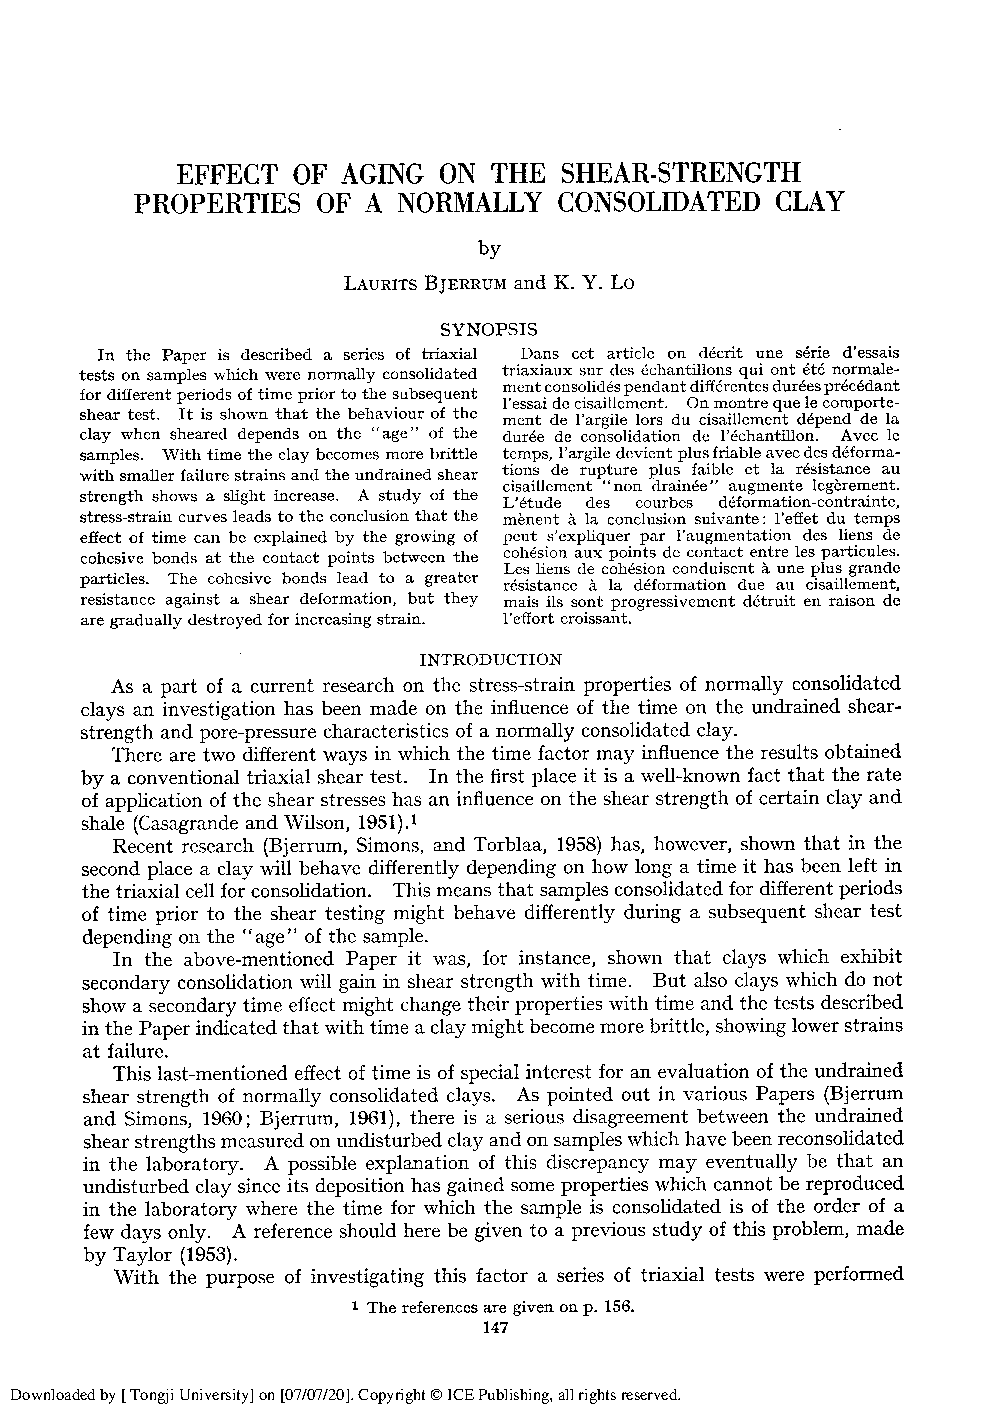
\includepdf[pages=1-11]{Bjerrum and Lo - Effect of Again of the Shear-Strength Properties of a Normally Consolidated Clay.pdf}

\end{document}